\subsection{Candidate-Pool Size and Token Usage}
\label{app:candidate-pool-tokens}
Figure~\ref{fig:performance_token_usage_by_topk} compares three measured candidate-pool sizes for Qwen3.5 4B with SkillSight. Here, $K$ is the number of retrieved candidates evaluated by the router, not the selected skill budget. Each run completed ten optimization iterations, and quality is measured on the final policy over 748 test tasks. The aggregate nDCG@10 is task-instance weighted rather than an equal-weight mean over datasets.

At $K=10$, final nDCG@10 is 0.702 with 692.788 million known tokens; at $K=25$, it is 0.742 with 1013.401 million; and at $K=50$, it is 0.800 with 1324.251 million. Across these three settings, higher observed routing quality accompanies higher recorded token use. This comparison describes the observed quality--cost tradeoff; it neither isolates a causal effect of candidate-pool size nor establishes a generally optimal setting.

All candidate-pool configurations use the same initial predicates. Totals cover recorded run-local usage and omit usage that is unavailable. They are not full token accounts or per-query serving costs, and these runs do not provide a controlled, budget-matched comparison.

\begin{figure*}[!t]
\centering
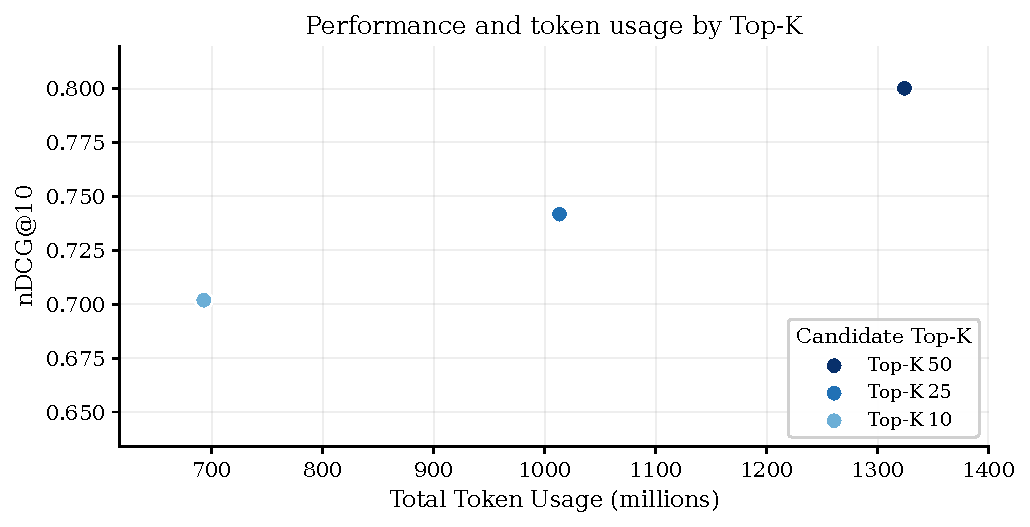
\includegraphics[width=\linewidth]{figs/performance_token_usage_by_topk/preview.pdf}
% The plain-text description contains literal underscores (n_tasks).
\begingroup
\catcode`\_=12
\caption[Recorded tokens and routing performance at different candidate-pool sizes.]{\input{figs/performance_token_usage_by_topk/description.text}}
\label{fig:performance_token_usage_by_topk}
\endgroup
\end{figure*}

